
\section{Conflict in Reasoning}\label{sec:ch7-conflict}

It is clear, both from this thesis and from a wealth of previous work
\citep{DeNeys2012,Crisp-Bright2010,Botvinick2004a,Miller2001},
that conflict in cognition arises in many places.
In Chapter 1, I introduced two particular junctures:
conflict between competing representations in induction,
and conflict between Type 1 and Type 2 processes.
At this point, it is worthwhile considering
how these two forms of conflict fit into
the broader scope of the interacting processes
that underlie reasoning.

I propose that
both kinds of conflict
can be understood in terms of
the role of working memory in reasoning,
and the interaction of working memory-based processes
with other cognitive processes.

Some cognitive functions
are almost certainly achieved by
fast, associative, processes.
Typical, but not defining properties of these processes are that
they are autonomous (they operate automatically
when presented with their triggering cues),
they are associative (rather than rule-based),
they generally operate quickly,
and are not cognitively demanding.
In dual process accounts of cognition,
these are known as Type 1 processes
\citep[or, in the past, as \emph{System 1}; e.g.][]{Sloman1996}.
\citet{Stanovich2005,Stanovich2009}, highlighting the diversity of these processes,
labels them the \emph{Autonomous Set of Systems}.
In his definition of this set of processes,
\citet{Stanovich2009} includes
both domain specific evolved \emph{modules},
and general learned associations,
which have become autonomous through practice or repeated exposure.
While some of these Type 1 processes serve to
provide information to other cognitive process,
including for use in more effortful, deliberate cognition,
others can affect our actions directly
without being mediated by other processes.


Clearly, under this definition, many cognitive processes are autonomous.
To fully catalogue these processes would take a lifetime,
and so for the purpose of this discussion
it suffices to say that there exist a constellation of processes
that are generally fast, associative, and autonomic.
Well-known such processes include face recognition
\citep[largely an evolved processes,
  localised to the fusiform gyrus;][]{Kanwisher1997},
reading text \citep[a learned skill
  that maps onto the left fusifom gyrus;][]{McCandliss2003},
and word recognition \citep[e.g.][]{Spivey2005}.

%% %% %% %% %% %% %%% 
%% Here be Dragons %% 
%% %% %% %% %% %% %%% 

%% Aidan: given John's concerns, I think that you need something here
%%    where you first talk about Type 2 processes and how the thing that
%%    distinguishes them from Type 1 processes is that they rely on Working
%%    Memory. The importance of WM to current dual process frameoowrks will
%%    allow you to attempt to resolve the various findings in your
%%    thesis....and then you can proceed from there. Otherwise, John is
%%    right, you look like you are taking a theoretical turn that you
%%    haven't advertised or prepared the reader for.

%% 

%% \aside{From Evans and Stanovich (2013)
%%   The definition of Type 2 processing:
%%   The large literatures on working memory and executive function
%%   (Baddeley, 2007) have established that there is a general purpose
%%   system used in many higher cognitive functions and that the capacity
%%   of this system varies reli- ably between individuals. [\ldots]  It is
%%   the engagement of this system specifically that Jonathan Evans
%%   (e.g., 2008, 2010a) has emphasized in the definition of Type 2
%%   processing and which underlies many of its typically observed
%%   correlates: that it is slow, sequential, and correlated with
%%   measures of general intelligence. [\ldots]  Stanovich (Stanovich, 2011;
%%   Stanovich \& Toplak, 2012) has also strongly emphasized the features
%%   that he calls “cognitive decoupling” in his definition of Type 2
%%   processing. This is again compatible with Evans’s (2007a, 2010b)
%%   view that such processing is necessary for hypothetical thought. In
%%   order to reason hypothetically, we must be able to prevent our
%%   representations of the real world from becoming confused with
%%   representations of imaginary situations. The so-called cognitive
%%   decoupling operations are the central feature of Type 2 processing
%%   that makes this possible according to Stanovich (2009b, 2011).
%% }

%% \aside{
%%   The definition of Type 1 processing: 
%%   We both agree that the defining characteristic of Type 1 processes is
%%   their autonomy. They do not required ``controlled attention'', which
%%   is another way of saying that they make minimal demands on working
%%   memory resources.}
%% 
%% }

Other processes, however,
require the sustained representation,
maintenance, and manipulation of information in working memory,
\emph{decoupled} from interference from
competing Type 1 processes \citep{Stanovich2008,Evans2013a,Gilbert1991}.
More recent dual process accounts
\citep[see][]{Evans2013a,Stanovich2012,Evans2004}
propose that this decoupling in working memory
is the defining feature of Type 2 processes.
In this account, Type 1 processes, in contrast,
are simply those that are \emph{autonomous},
or do not require controlled attention or working memory resources
\citep[p. 236]{Evans2013a}.

These Type 2 processes,
making use of working memory,
have the advantage of being extremely flexible.
Many Type 1 processes are thought to be \emph{domain specific} \citep[see][]{Cosmides1994a},
in that they are restricted to processing only one kind of information.
An archetypal example of this is the process responsible for face perception,
a small system localised to the bilateral fusiform gyri
\citep[or \emph{fusiform face areas; }see][]{Kanwisher1997}.
This system is exquisitely well adapted to recognise human faces in visual input,
but when presented with other stimuli will either not activate,
or mistakenly indicate that it has seen a face.%
\footnote{
  The common illusion of perceiving faces
  in non-facial stimuli is known as pareidolia.}
Type 2 processes, however, are \emph{domain general},
and can equally well process information about faces, words,
geographical locations, and abstract concepts.
These processes are also thought to be unique
in their ability to sequentially apply rule-based operations
\citep{Cooper1973,Anderson2014,Anderson1996a},
in contrast to Type 1 processes, which are thought to
work on associative principles \citep[see][]{Sloman1996}.
This flexibility comes at the cost, however, of limited capacity.
Working memory capacity
--- and thus the capacity of Type 2 processes ---
is limited first of all in that, compared to Type 1 processes,
through which an enormous amount of information streams in parallel,
only a very small amount of information can be held
in working memory at one time
\citep[famously 7 chunks of information, $\pm$ 2, according to][]{Miller1956}.
Working memory is limited secondly in that
many theories hold that only one state of the world,
or mental representation,
can be held in working memory at any one time.
This means that we can consider one possible mental representation,
followed by another, but that we cannot simultaneously consider
two contradictory representations.
This limitation has been noted across a number of research traditions,
including in dual process theories as the
\emph{singularity principle} \citep{Evans1984,Evans2006},
in mental models accounts of reasoning \citep{Johnson-Laird1983}
as \emph{focusing} \citep{Legrenzi1993},
by those interested in diagnosis as an inability to
consider more than one hypothesis at a time \citep{Mynatt1993},
as well as in the literature on working memory itself \citep{Baddeley2007}.

My proposition is as follows.
First, the inductive triad tasks used in Chapters 3 and 4
require that participants hold
the three categories presented in working memory,
to compare the inductive potential from the base
to each of the candidate responses.
To do this, they must draw on information
about the relationships between the categories shown.
This information, naturally, must come from elsewhere,
and in these tasks it can come from a number of Type 1 processes:
from the visual system, for instance,
or from different aspects of long term memory \citep{Jackson2015},
including both associative and structured knowledge.
As only one representation of the world
can be held in working memory at a time,
conflict arises when multiple Type 1 processes
provide multiple contradictory representations.
I contend that the induction tasks reported here
involve conflict in this sense,
as representations based on perceptual cues or conceptual knowledge
(Experiments 1 and 2),
or on associative and structured knowledge (Experiments 3 and 4)
vie to be realised.

Second, there are some problems for which responses can be cued
either by Type 1 processes,
operating on associative principles and placing few demands on working memory,
and by Type 2 processes
that involve maintaining information in working memory
while applying sequential, rule-based operations.
These are, of course, the problems addressed by
dual process theories of reasoning.
\citep[e.g.][]{Evans2013a,Evans2008,Kahneman2011}.
I investigated two such problems in this thesis:
reasoning about base rates and stereotypes (Experiments 5),
and the Cognitive Reflection Test (Experiment 6).
My account for performance on these tasks
is no different from the generic dual process account.
On the base rate task, Type 1 processes
are responsible for processing the descriptions,
and automatically cue stereotype-consistent responses.
To process and respond on the basis of the base rates, however,
one must engage Type 2 processes to relate
the statistical information to the task at hand and choose a response
(and, under most accounts, to inhibit the description-cued response).
Similarly, on the CRT,
Type 1 processes automatically cue incorrect heuristic responses,
without the need for sustained Type 2 processing.
To reach the correct response, however,
participants must represent the problem in working memory
and apply the rules of arithmetic, an archetypal Type 2 operation.

\begin{figure}[ht]
  \centering
  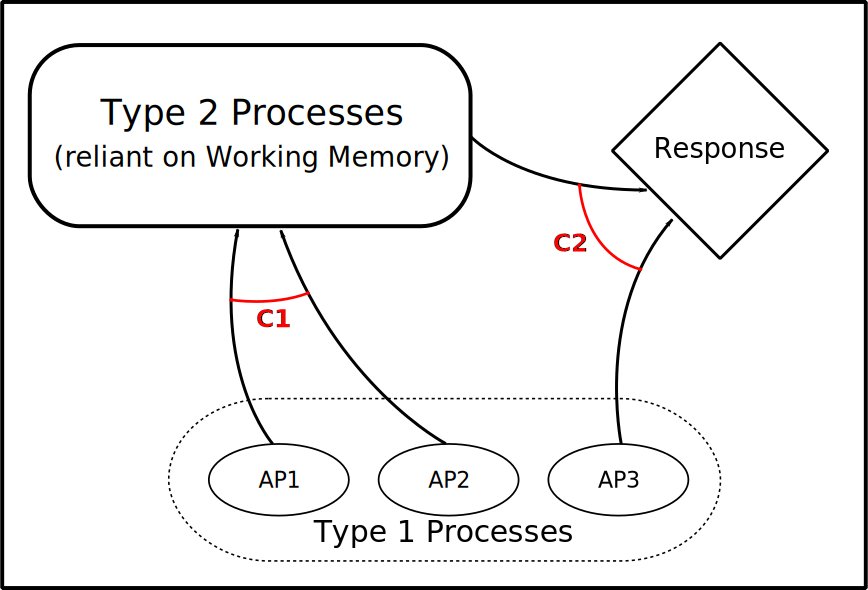
\includegraphics[width=\figurewidth]{imgs/simple-framework.pdf}
  \caption[A framework for conflict in reasoning]{
    \label{fig:conflict-framework}
    A simple framework for conflict in reasoning.
    Reasoning requires the interaction of
    associative, Type 1 processes (AP1, AP2, AP3, etc.),
    and Type 2 processes, reliant on working memory.
    Conflict in reasoning arises
    a) when multiple Type 1 processes
    attempt to project information to working memory
    (\textcolor{red}{C1}), and
    b) when both Type 1 
    and Type 2 processes attempt to produce responses
    (\textcolor{red}{C2}).
    I propose that conflict of type \textcolor{red}{C1} occurs
    when multiple sources of information,
    such as perceptual cues, associative knowledge, or structured knowledge,
    are available during inductive reasoning.
    Conflict of type \textcolor{red}{C2}, conversely,
    occurs in reasoning when both Type 1 and Type 2 processes
    can generate responses, for instance description
    and base rate-cued responses in Experiment 5,
    or heuristic and correct responses in Experiment 6.
  }
\end{figure}

Figure~\ref{fig:conflict-framework} shows a simple sketch of
this framework for thinking about conflict in reasoning.
In short, conflict can arise both
as multiple Type 1 processes attempt to project information to working memory,
or because both Type 1 and Type 2 processes
attempt to produce responses to the same problem.
With this framework in mind, I now return to the interpretation of my results.
